%=== CHAPTER TWO (2) ===
%=== Literature Review ===

\chapter{A Literature Review}
\label{cha:literature}
\begin{spacing}{1.5}
\setlength{\parskip}{0.3in}

This chapter will review the theory basis related to lane detection. \autoref{sec:LR_overview} briefly reviews the development in the lane detection area from two perspectives: the classical one and the deep-learning one. \autoref{sec:LR_NNB} compares the machine learning and different types of deep-learning and describe the neural network working mechanism from the foundation. This section also explains how the back-propagation/feed-forward/neutron-calculation works with clear diagrams. \autoref{sec:LR_FCN} describes how the Fully Convolutional Network work and its advantage. Especially, it describes how the convolutional layer is related to neutrons, to which even many textbooks do not give the detail.

\section{An Overview}
\label{sec:LR_overview}

The lane detection method has been developed from classical ones to novel deep-learning-based ones in the past few years. This section will give a brief review of the classical lane detection methods proposed and give a brief overview of the developments of object detection.

\subsection{Classical Lane Detection}

There are several ways to get the information for lane detection and prediction usages, such as Monocular vision, stereo, LIDAR, inertial measurement unit (IMU) combined with information obtained from global positioning system (GPS) and high-resolution digital maps. \cite{hillel2014recent}. This dissertation focuses on Monocular vision (Single camera).

As classical approaches, some researchers used Inverse Perspective Mapping (IPM) to recover a bird's-eye-view image. The lane pictures captured by in-vehicle cameras have the problem of distorted perspective, thus a perspective transformation is needed to recover the overlooking perspective like in birds' eyes~\cite{luo2010low}. In a work in 2010, researchers used IPM to remove the fisheye distortion and implement obstacle detection~\cite{lin2010construction}. They developed a quick searching scheme to analyse the object in each direction utilizing a polar histogram. However, this method is limited at obstacle's shape; thus, not efficient in lane detection.

In previous work, researchers found a relationship between wheeling and gaze direction when driving. Human employs the distant region to estimate the road curvature \cite{land1995parts}. Also, the gaze direction relies on the `tangent point' on the inside of each curve when driving on the curvature of the road ahead \cite{land1994we}. This gives possible to utilize the unseen vanishing point in lane prediction.

\subsection{Deep-learning based Lane Detection}

Lane and road marking detection tasks are within the scope of object detection, so algorithms popular in object detection have been implemented in lane detection \cite{tang2020review}. 

Object detection is the process to determine whether the instances of objects exist in image~\cite{liu2020deep}. Object detection can be stated as two different tasks: specific object detection, which detects unchanged certain object~\cite{zhang2013object}, such as Barack Obama’s face, MacBook Pro, and Eiffel Tower; and generic object detection, which detect all the objects in a general category (have been seen or unseen before), such as lanes, road markings, and dogs. 

In recent years, with the DCNN like AlexNet \cite{krizhevsky2012imagenet} being brought up, deep learning has been driving significant progress in the object detection area. Later RCNN and its variants \cite{girshick2014rich, girshick2015fast, ren2015faster} integrates CNN with the region proposal selective search; GoogLeNet \cite{szegedy2015going} and VGGNet \cite{simonyan2014very} gained improvement with deeper encoder. With the network going deeper, computational efficiency becomes the main problem. More powerful network architectures such as ResNets \cite{he2016deep}, DenseNets \cite{huang2017densely}, and Inception \cite{ioffe2015batch} have been proposed, which combine path blocks to reduce the number of parameters while improving the accuracy. Most recently, DETR \cite{carion2020end} combined the CNN with transformer architecture, taking the object detection problem as a set-set mapping and achieved promising results on big-object detection.

Lanes are thin and small objects; thus, general methods sometimes work poorly \cite{tang2020review}. There are some researches featured in picking out tiny items. U-Net \cite{ronneberger2015unet} extracts the feature map from the encoding path and attach it to the decoding path (or in other words, the encoding and decoding paths are shortcut by a skip path), encourage the shorted layer to learn residuals instead of directly learning features. The U-Net is hot in segmentation area for its ability in contextual sensing and high-resolution segmentation, and is possible to be extended to object detection.

Efforts to use the neural network in lane detection tasks have also been proved solid. Work \cite{borji2016vanishing} first used the CNN structure to predict the vanishing point, and VPGNet \cite{lee2017vpgnet} employed vanishing point information by multi-task method to enhance the prediction of the lanes.

\section{Neural Network Basis}
\label{sec:LR_NNB}

Neural Network is the most distinguished deep learning architecture based on Neural units (neurons) in recent years. Compared with conventional machine learning and human-designed mathematical classification algorithms, deep learning on the Neural Network have many advantages. This section will give the theoretical basis of the Neural Networks and explain how it works by introducing the backpropagation mechanism.

\subsection{Machine Learning}

Compared with specific mathematical equations designed for different kinds of problems, conventional machine learning is based on \textit{experience}. \textit{Experience} here means that: the machine learning computational models can learn the features from a given data set (learn the \textit{experience} from input), and do prediction or classification based on that \textit{experience} for any inputs, whether the new input data has been seen or unseen before.~\cite{mohri2018foundations}.

The process of learning the features can be seen as a clustering operation. Each input data can be mapped into a $n$-dimension vector, and each vector can be viewed as a point in the $n$-dimension hyperspace. \autoref{fig:2dcluster} and \autoref{fig:3dcluster} shows the $2D$ and $3D$ clustering process. Clustering is to group data points into different clusters in the hyperspace and draw the hyperplane between such clusters. This hyperplane is the interface between classes. For example, in figure \autoref{fig:2dcluster}, two data groups were divided by a linear line. In figure \autoref{fig:3dcluster}, two groups of data were divided by a non-linear curved surface.

\begin{figure}[ht]
\centering
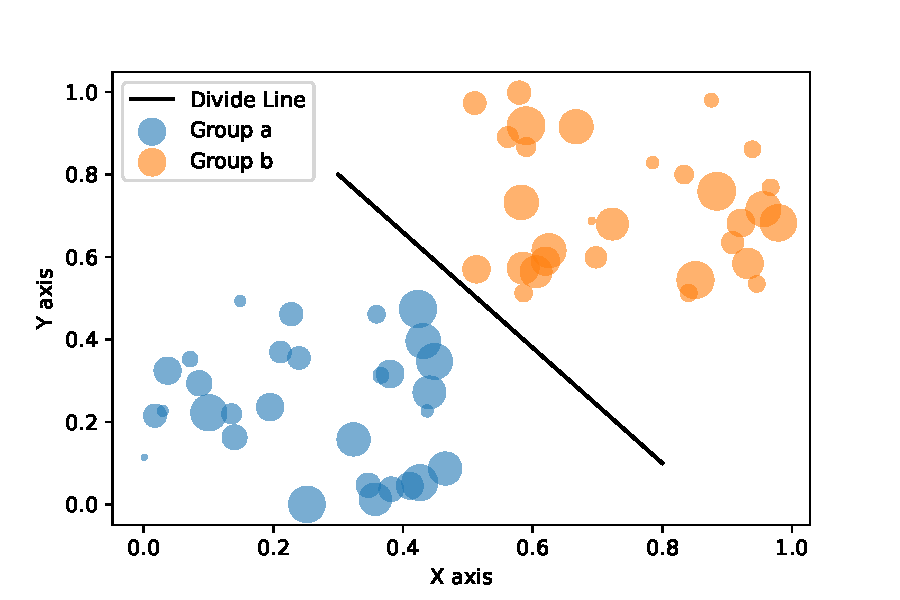
\includegraphics[width=0.99\textwidth, fbox]{Chapter2/2dcluster.pdf}
\caption{$2D$ Clustering}
\label{fig:2dcluster} 
\end{figure}

% \begin{figure}[ht]
% \centering
% \fbox{
% \includesvg[width=0.97\textwidth]{Chapter2/3dcluster.svg}
% }
% \caption{$2D$ Clustering}
% % \label{fig:2dcluster} 
% \end{figure}

\begin{figure}[ht]
\centering
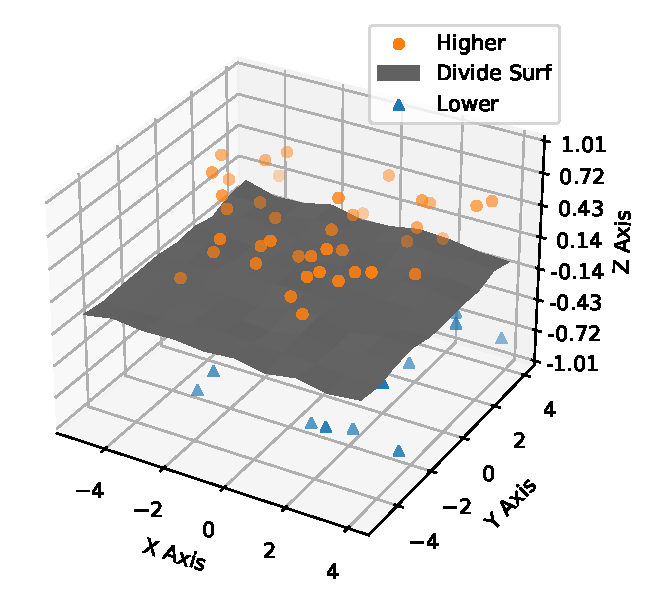
\includegraphics[width=0.6\textwidth, fbox]{Chapter2/3dcluster.pdf}
\caption{$3D$ Clustering}
\label{fig:3dcluster} 
\end{figure}

Above mentioned examples only calculate linear or non-linear division between two classes. Generally, in real-world applications, what is needed is not limited to binary classification but usually multi-classification. In machine learning, there are two solutions to the multi-classification problem: 

1) \textit{Uncombined algorithms} will treat the multi-classification as a whole and finish training in only one phase, such as $N$-class SVM, decision trees. 

2) \textit{Aggregated algorithms} will split $N$ class classification into many binary classification, thus need multiple training phase. There are two types of aggregated algorithms: a) \textit{One-versus-one} calculate boundaries for every pair of classes, thus for $N$ class, it needs $N!=N*(N-1)*...*2*1$ calculations, as shown in \autoref{fig:121}. b) \textit{One-versus-others} calculate the boundary between the target class and all other data, thus for $N$ class, it needs to calculate $N$ boundaries, as shown in \autoref{fig:12all}. 

\begin{figure}[th]
    \centering
    \begin{subfigure}[b]{0.49\textwidth}
        \centering
        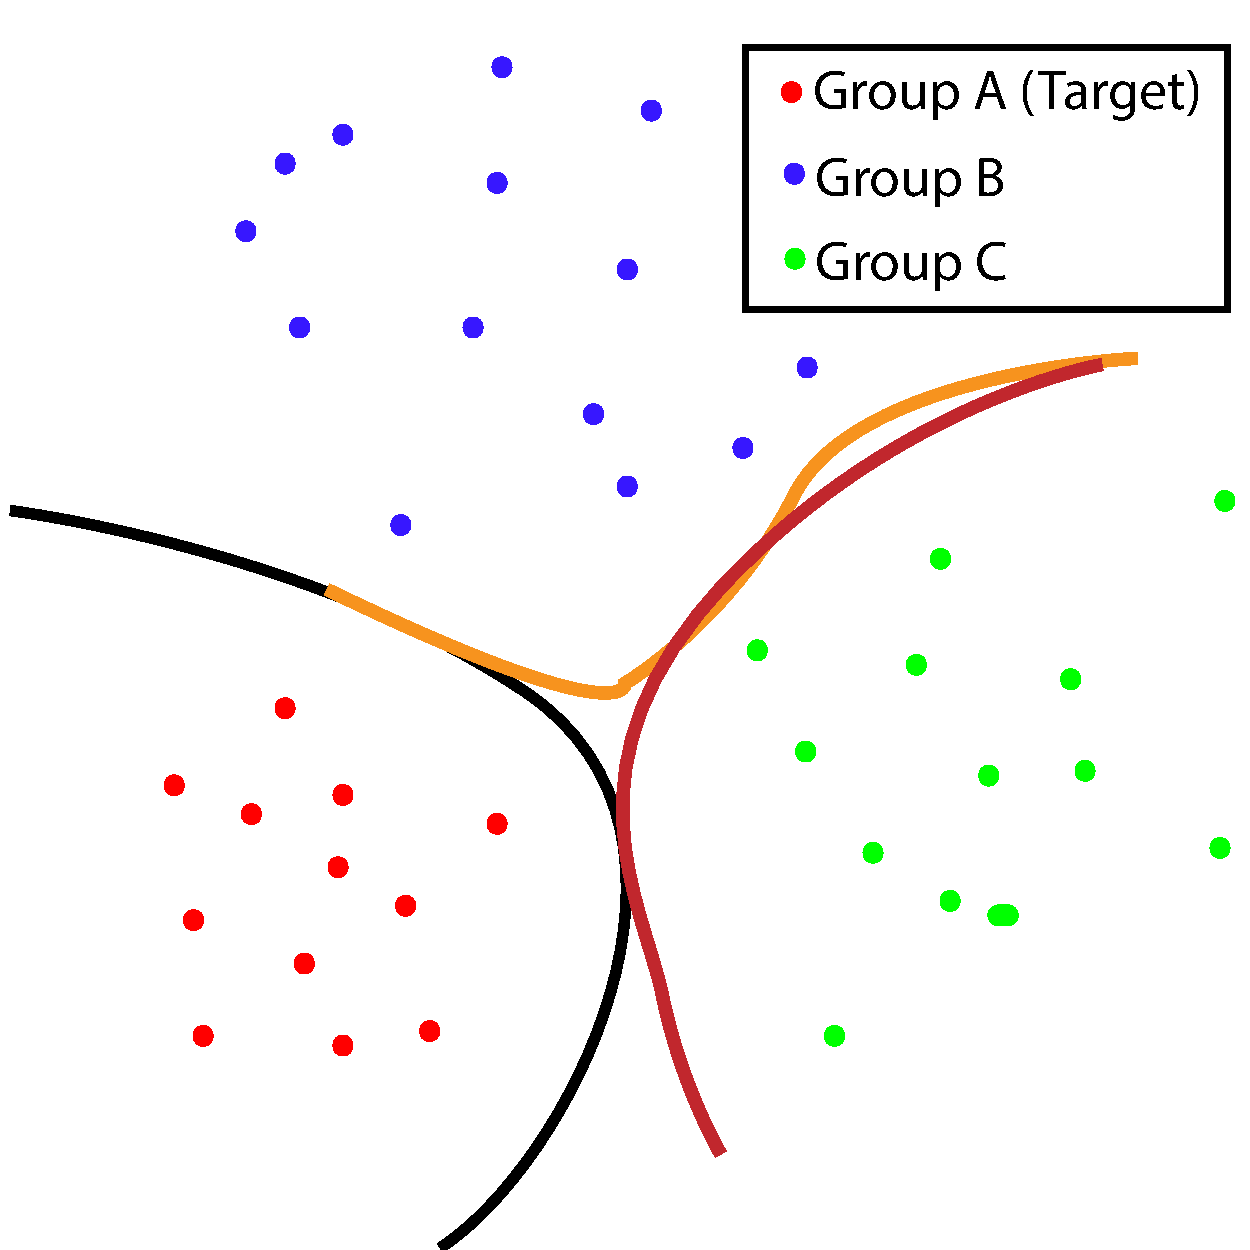
\includegraphics[width=2.7in, fbox]{Chapter2/1to1.pdf}
        \caption{One-to-one Multi-classification}
        \label{fig:121} 
    \end{subfigure}%
    ~
    \begin{subfigure}[b]{0.49\textwidth}
        \centering
        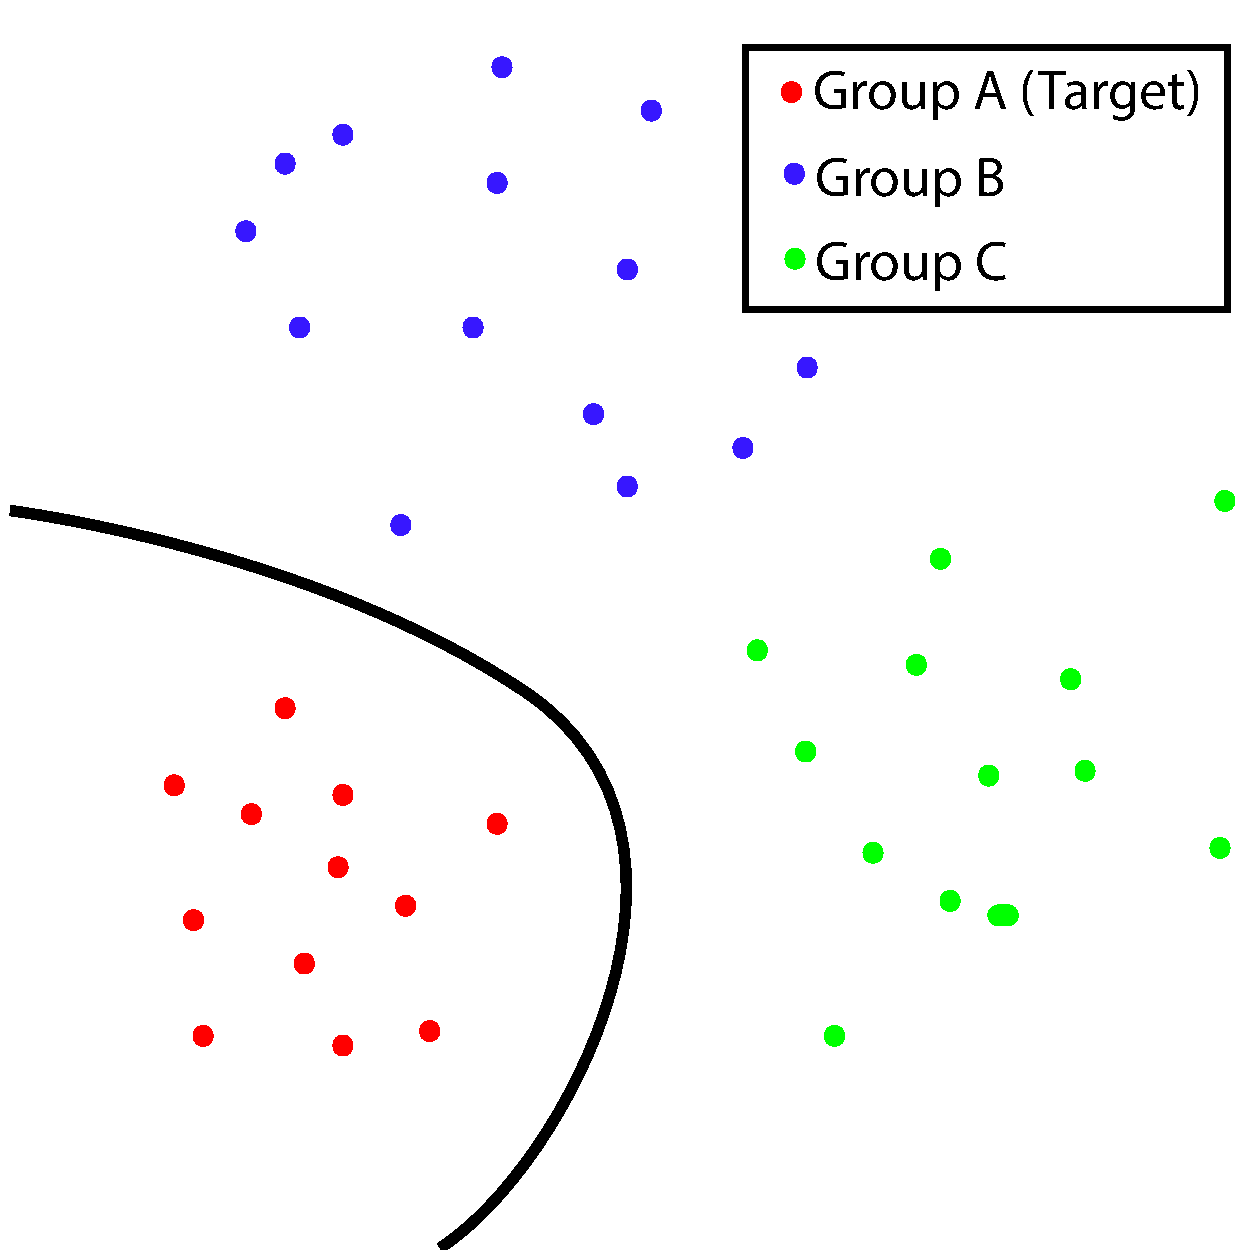
\includegraphics[width=2.7in, fbox]{Chapter2/1toall.pdf}
        \caption{One-to-all Multi-classification}
        \label{fig:12all} 
    \end{subfigure}
    \caption{Two Aggregated Algorithms}
\end{figure}


\subsection{Representation Learning and Deep Learning}

The main drawback of conventional machine-learning techniques is that they can not extract the features automatically and precisely from the raw input data. When using machine learning, engineers and researchers have to transform the raw data into normalized vectors that are suitable for training~\cite{ongsulee2017artificial}. From the normalized vectors, the machine learning model can classify and do detection on the classify patterns.

Representation learning allows the machine to discover the best representation form of the raw data for machine learning training. Representation learning features that the algorithm can find and fit the best representation from the raw input data, no matter what format the input data is. Such representation of raw data is suitable for the further feature extraction~\cite{bengio2013representation}. For example, if the input is a gray-scale image, the output matrix would represent the position of edges and corners after the first representation layer.

\begin{figure}[th]
    \centering
    \begin{subfigure}[b]{0.99\textwidth}
        \centering
        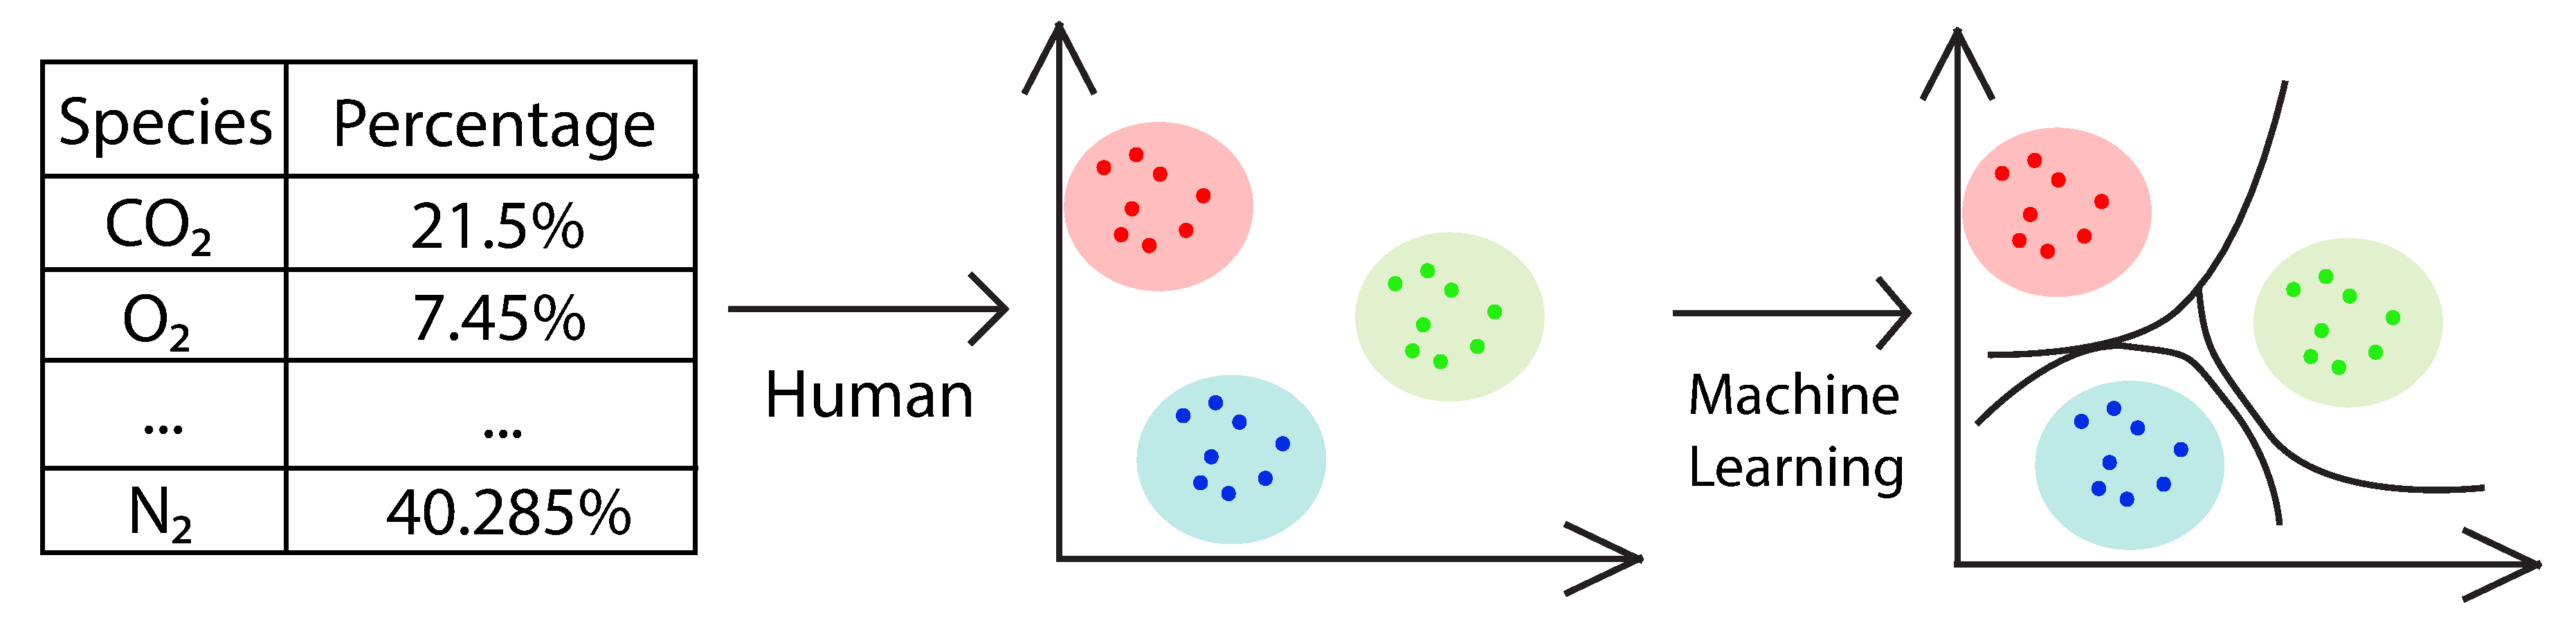
\includegraphics[width=0.98\textwidth, fbox]{Chapter2/Machine-Learing.pdf}
        \caption{Machine Learning: Human Data Centering}
        \label{fig:mldiagram} 
    \end{subfigure}%
    \\
    \begin{subfigure}[b]{0.99\textwidth}
        \centering
        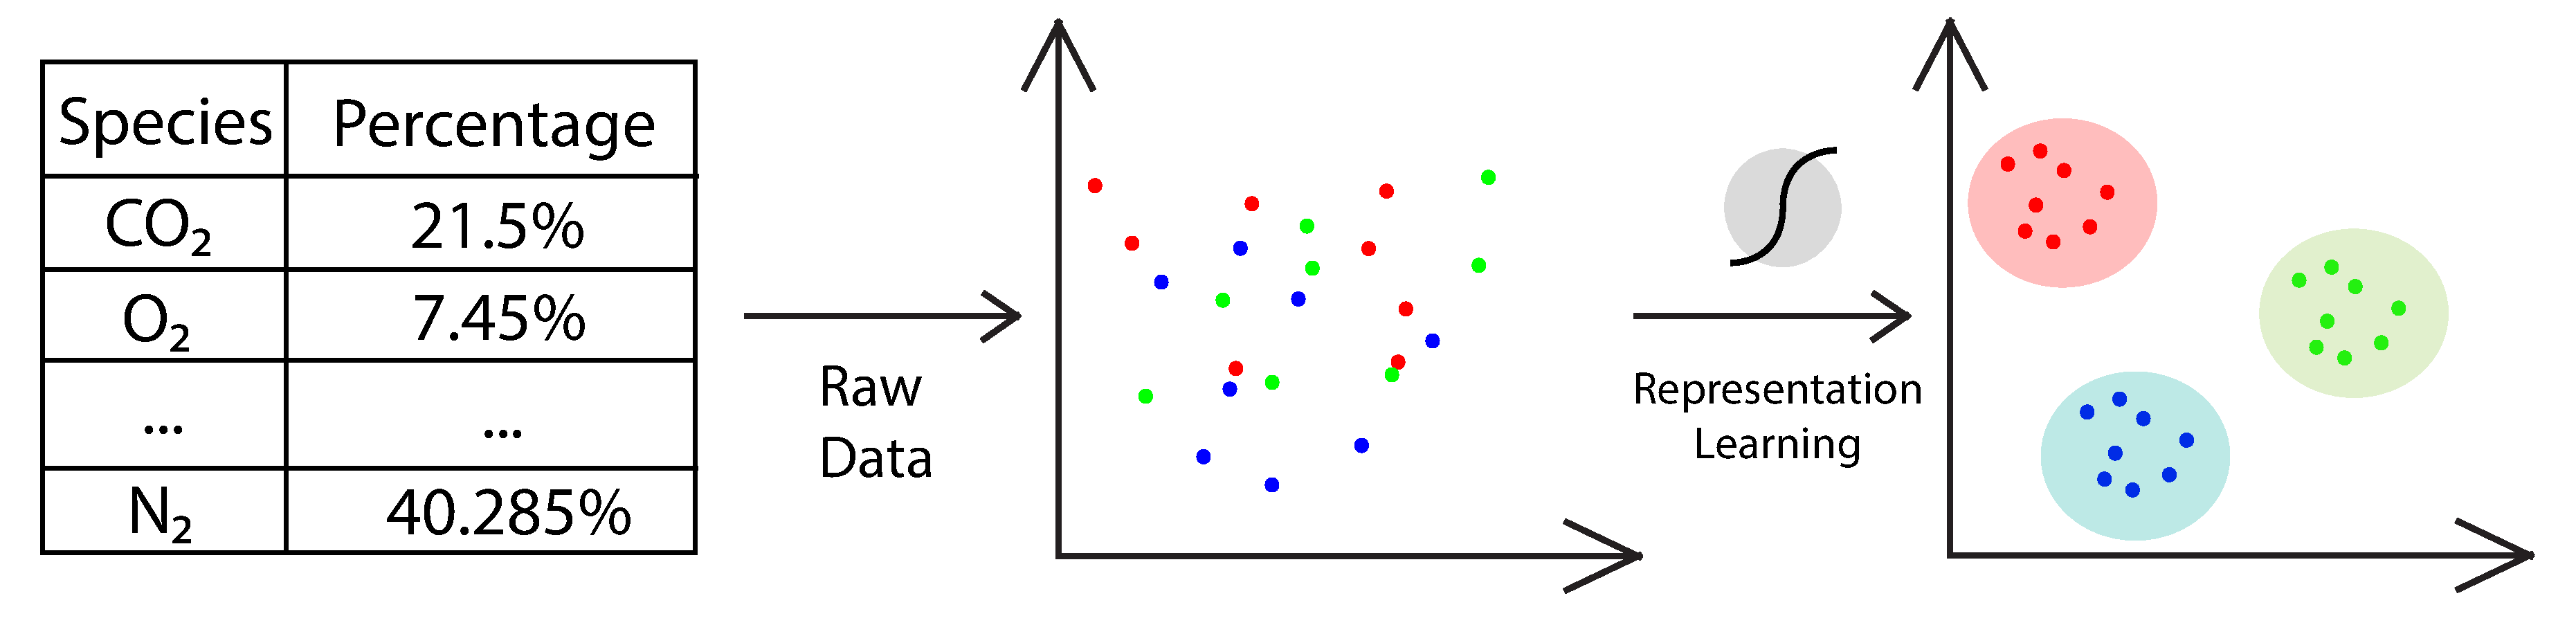
\includegraphics[width=0.98\textwidth, fbox]{Chapter2/Represent-Learing.pdf}
        \caption{Representation Learning: Auto Extraction}
        \label{fig:representdiagram} 
    \end{subfigure}
    \\
    \begin{subfigure}[b]{0.99\textwidth}
        \centering
        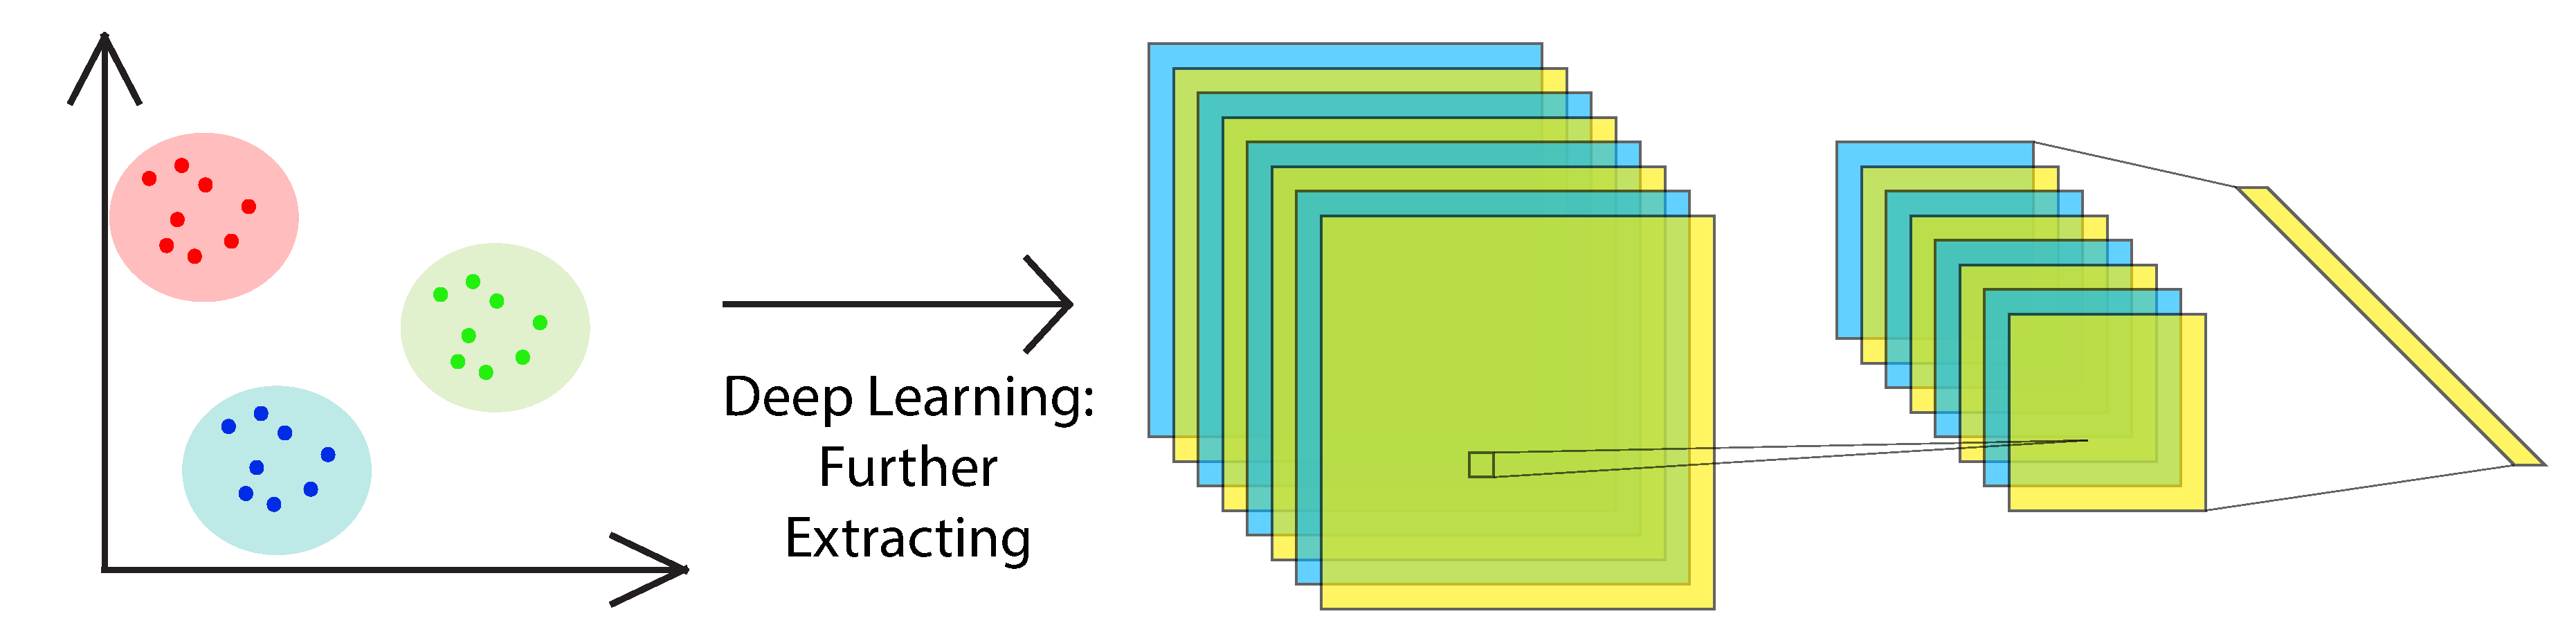
\includegraphics[width=0.98\textwidth, fbox]{Chapter2/Deep-Learing.pdf}
        \caption{Deep Learning: Further Extraction of Features}
        \label{fig:dldiagram} 
    \end{subfigure}%
    \caption{Comparison between Three Learning}
\end{figure}

Based on representation learning, the concept of deep learning was initially being proposed in a study on Artificial Neural Network (ANNs) \cite{hinton2006reducing}. Deep learning is a multi-layer and deeper version of representation learning. Deep learning can not only extract the feature vectors from the first layer but also can go deeper, get more abstract high-level features. For example, if the input is a gray-scale image, the first layer of deep learning is just like representation learning, extracting the position of edges and corners. The second layer of deep learning would extract the relative positions between the edges and corners, and the third layer of deep learning would treat edges and corners in similar shapes as a group. With the network go deeper, such high-level abstract features can be sensed. In 2006, with a deep learning architecture called deep belief network (DBN) \cite{hinton2006fast} being invented by Hinton, the machine learning community rekindled heated discussion over deep learning.

Give an example to illustrate the difference between machine learning, representation learning, and deep learning. For a chemical substances classification task, the input is the percentage of each component in a chemical mixture. Researchers have to re-form and normalize the input data into a sparse data space when using machine learning algorithms like SVM. They should do multi-phase training for multi-classification (\autoref{fig:mldiagram}). When using representation learning methods, the input data can be raw data that has not been pre-processed (\autoref{fig:representdiagram}). Such raw data will be mapped to high-dimension space by non-linear network basic units (the Neurons). When using deep learning, the extracting layer goes deeper, thus can get more abstract features (\autoref{fig:dldiagram}).

Deep learning~\cite{lecun2015deep} is composed by simple non-linear \textit{Neuron} in each level. \textit{Neuron} is described in \autoref{subsec:neural_unit}. Deep learning uses the back propagation and feedforward mechanism to optimize the non-linear parameters of \textit{Neuron} from front to end. Propagation and feedforwad are described in \autoref{subsec:back_propagation}.


\subsection{Supervised, Unsupervised and Reinforcement Learning}

Machine learning algorithms can be classified into three main categories, according to the training data form and the algorithm's learning mechanism: supervised learning, unsupervised learning, and reinforcement learning \cite{mohri2018foundations}. Between supervised learning and unsupervised learning, there is also semi-supervised learning.

Supervised learning is trained on labeled input and output~\cite{sen2020supervised, kotsiantis2007supervised}. Each input data $D_i$ is paired with a label or ground-truth value $L_i$. Thus the training data should be in the format: $(D_i, L_i), i \in \mathbb{Z}$. The supervised learning aims to predict the corresponding label $l_i$ for each new input $d_i$. Supervised learning can be divided into two types: 

\begin{enumerate}
    \item Regression, when the label set $\{L_i\} = \mathbb{R}$, in which $\mathbb{R}$ is continuous real number set.
    \item Classification, when the label set $\{L_i\} = \mathbb{A}$, in which $\mathbb{A}$ is a set of discrete values $\{\alpha_1, \alpha_2, ...\}$ representing different classes.
\end{enumerate}

 Unsupervised learning is to cluster unlabeled data set into different groups according to their statistical feature\cite{meena2019survey}. It analyzes the bounding of a given vector set $\{D_1, D_2, ...,D_n\}$ (the training data), finds the similarities in the observed attributes in the hyperspace, divides the set into $n$ groups $\{G_1, G_2, ..., G_n\}$, and tells if a new unseen data $d_i$ belongs to or not belongs to certain class $G_i$.

\begin{figure}[ht]
\centering
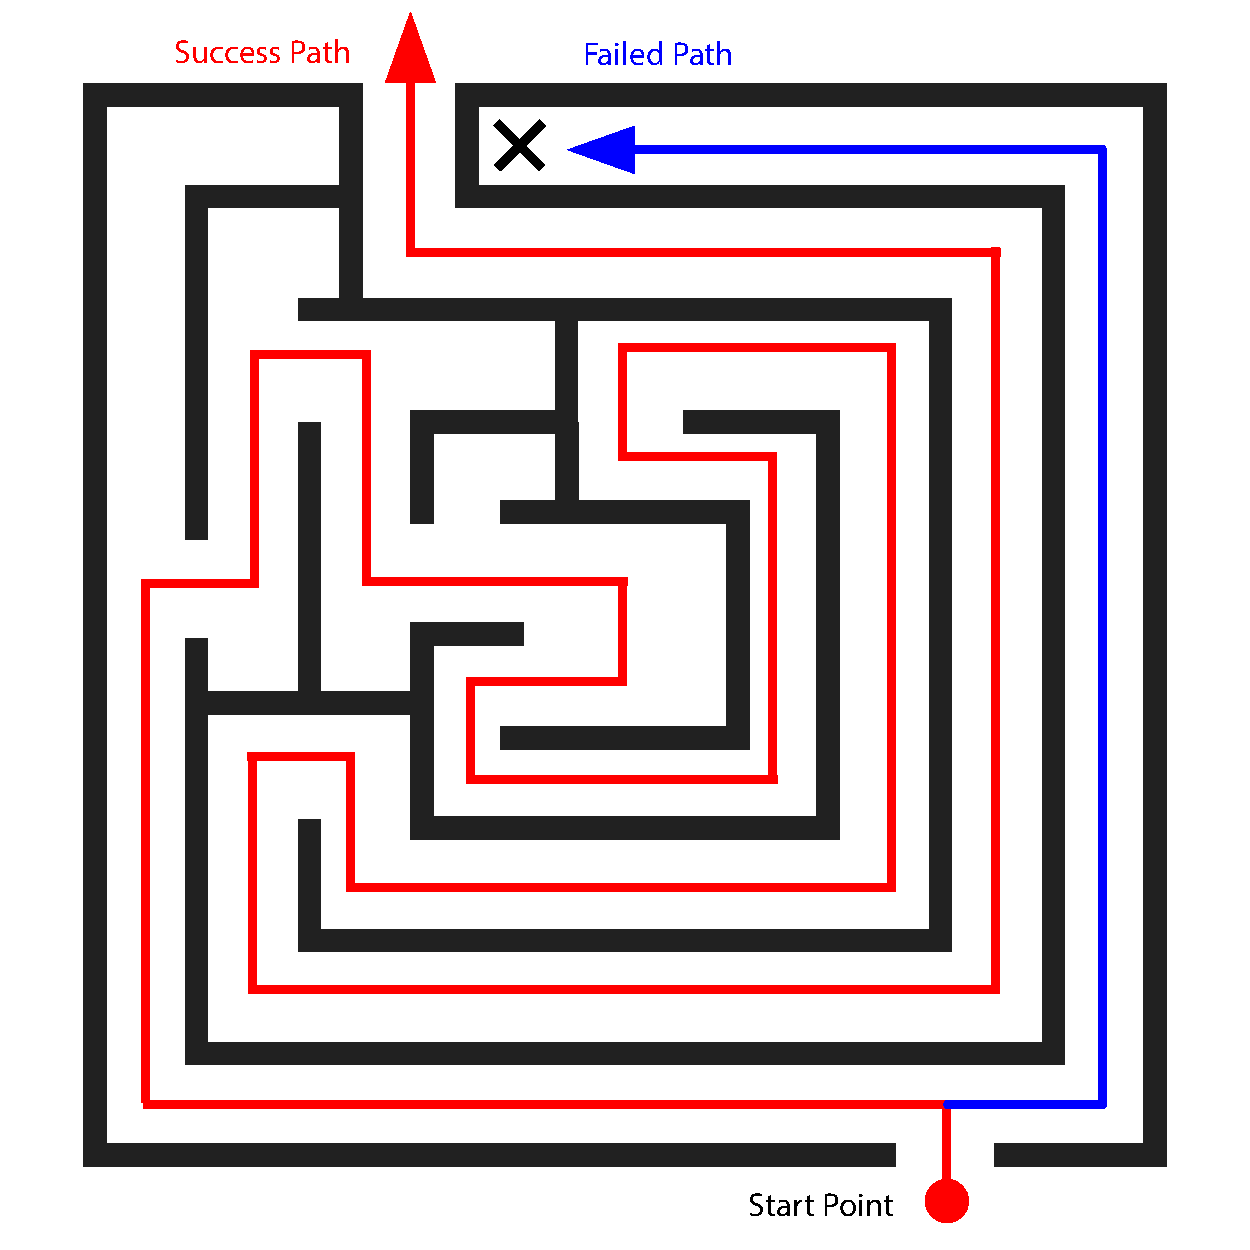
\includegraphics[width=0.75\textwidth, fbox]{Chapter2/reinforcement.pdf}
\caption{Reinforcement Learning: Maze Game Decisions}
\label{fig:reinforcement} 
\end{figure}

Reinforcement learning is to make the agent to play a game, or to perform a series of actions to reach to a certain goal~\cite{barto2004reinforcement}. The model will face a game-like situation, and make a consequence of decision to achieve the highest game score, as shown in~\autoref{fig:reinforcement}. First, the agent will observe the environment $\{\vec{E_i}\}$, which is a set of vectors representing the surrounding conditions. Second, the agent will conduct some action $\vec{a_i}$, and receive the reward/punishment score $\tau_i$. The aim of reinforcement learning is to find set of actions $\{\vec{a_i}\}, i \in (1,N)$, and such actions should satisfy the condition as described in~\autoref{eq:reinforce}.

\begin{equation}
\label{eq:reinforce}
   z = \argmax_{\{\vec{a_i}\}} \sum_{i=1}^{N} \tau_i
\end{equation}

Reinforcement learning is to make the agent play a game or perform a series of actions to reach a certain goal~\cite{barto2004reinforcement}. The model will face a game-like situation and make a consequence of decisions to achieve the highest game score, as shown in~\autoref{fig:reinforcement}. First, the agent will observe the environment $\{\vec{E_i}\}$, which is a set of vectors representing the surrounding conditions. Second, the agent will conduct some action $\vec{a_i}$, and receive the reward/punishment score $\tau_i$. Reinforcement learning aims to find a set of actions $\{\vec{a_i}\}, i \in (1,N)$, and such actions should satisfy the condition as described in~\autoref{eq:reinforce}.

\subsection{Network Unit: Neuron}
\label{subsec:neural_unit}

\begin{figure}[ht]
\centering
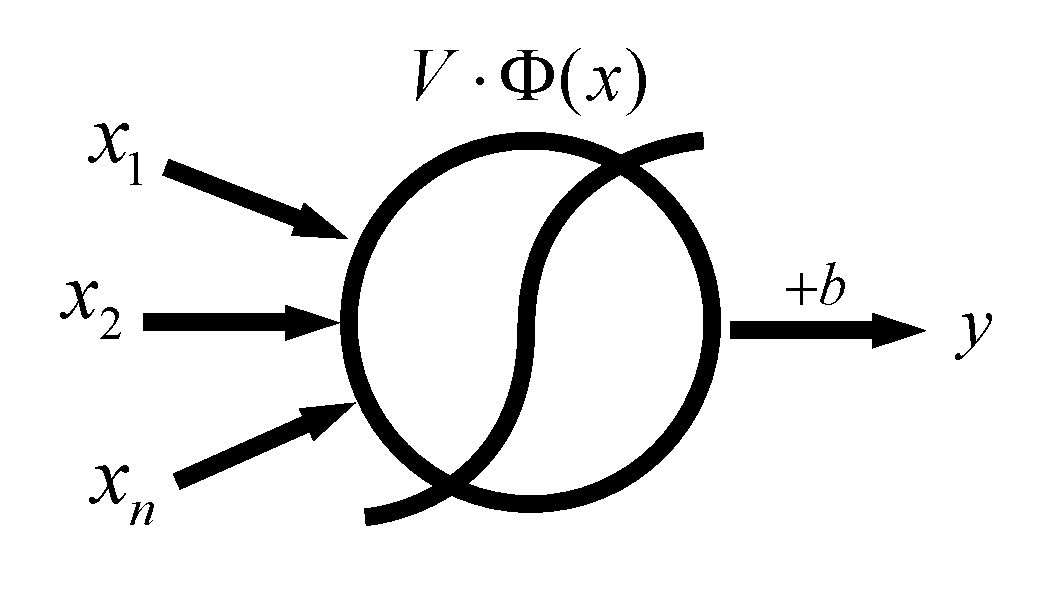
\includegraphics[width=0.5\textwidth, fbox]{Chapter2/neuralunit.pdf}
\caption{One Neuron}
\label{fig:neuralunit} 
\end{figure}

The most basic unit that constructs the neural network, the ``neuron", is relatively simple that is only a non-linear function with $n$ inputs and one output~\cite{bengio2017deep}, as shown in~\autoref{fig:neuralunit}. 

The function of input and output is as~\autoref{eq:neuralunit} shown. 

\begin{equation}
\label{eq:neuralunit}
    f(x)=b+V \cdot \Phi (c+W \vec{x})
\end{equation}

The $\vec{x_i},i \in [1,n]$ is the input value of the neutron. Usually, those input values are the direct output of the previous neutron. The $W_i$ is the weights for each input, which is also called the parameter in deep learning. These weights are the primary values deep learning try to adjust in the learning process . The $c$, $b$, and $V$ are constants, they are offset for input, output, and the scaling factor for the output. The $\Phi (\cdot)$ is the activation function, which could be some non-linear functions like \textit{Sigmoid} (\autoref{eq:sigmoid}), \textit{ReLU} (\autoref{eq:relu}) or \textit{Tanh} (\autoref{eq:tanh}). The image for the activation functions are shown in~\autoref{fig:activationfunc}. The activation function maps the input to another data space which is easier to perform classification. 



\begin{gather}
% \vspace{-0.3in}
   \Phi_{Sigmoid}(x)=\frac{1}{1+e^{-x}} \label{eq:sigmoid}\\
   \Phi_{ReLu}(x)=max(0,x) \label{eq:relu}\\
   \Phi_{Tanh}(x)=\frac{e^{x}-e^{-x}}{e^{x}+e^{-x}} \label{eq:tanh}
\end{gather}

\begin{figure}[th]
    \centering
    \begin{subfigure}[b]{0.49\textwidth}
        \centering
        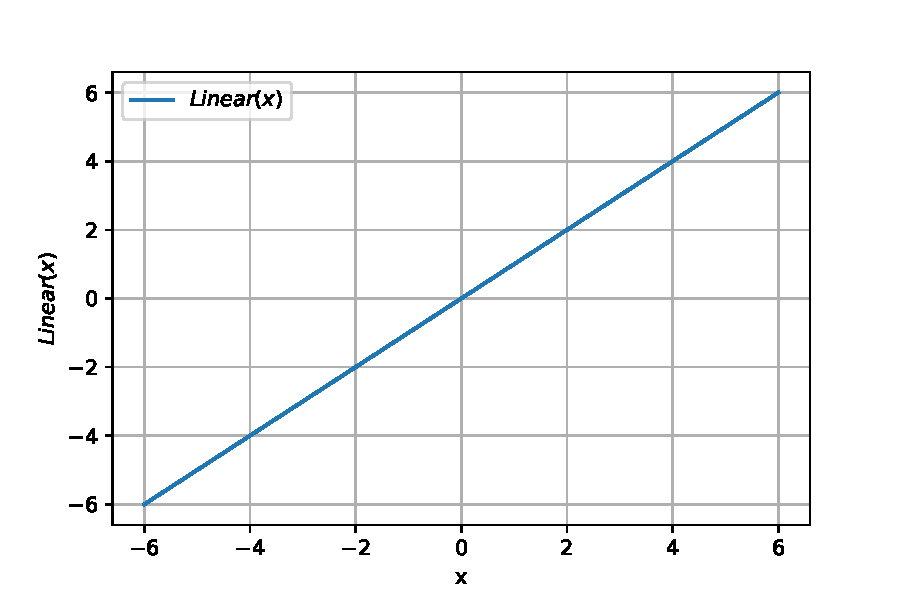
\includegraphics[width=2.7in, fbox]{Chapter2/linear.pdf}
        \caption{Linear}
    \end{subfigure}%
    ~
    \begin{subfigure}[b]{0.49\textwidth}
        \centering
        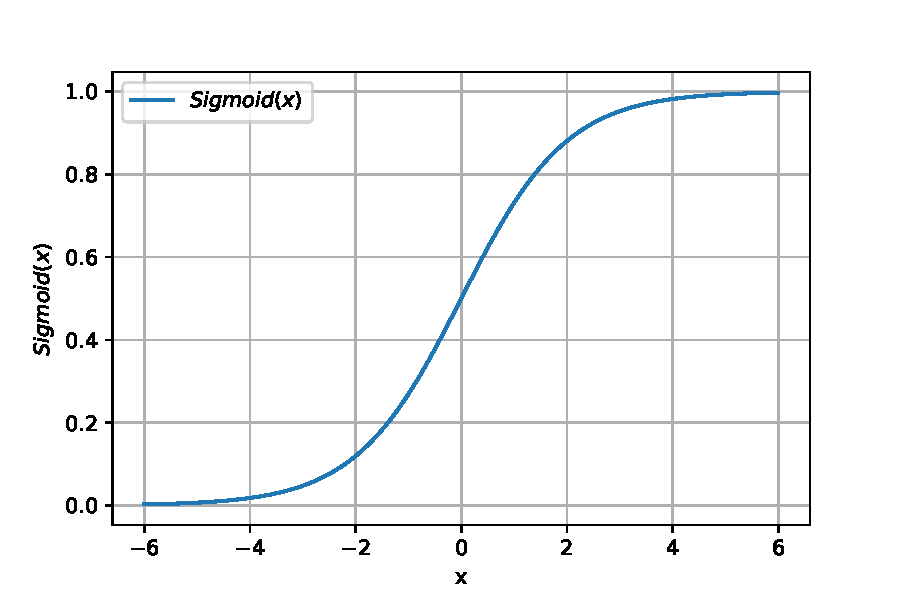
\includegraphics[width=2.7in, fbox]{Chapter2/sigmoid.pdf}
        \caption{Sigmoid}
        % \label{fig:sigfunc} 
    \end{subfigure}
    \\
    \begin{subfigure}[b]{0.49\textwidth}
        \centering
        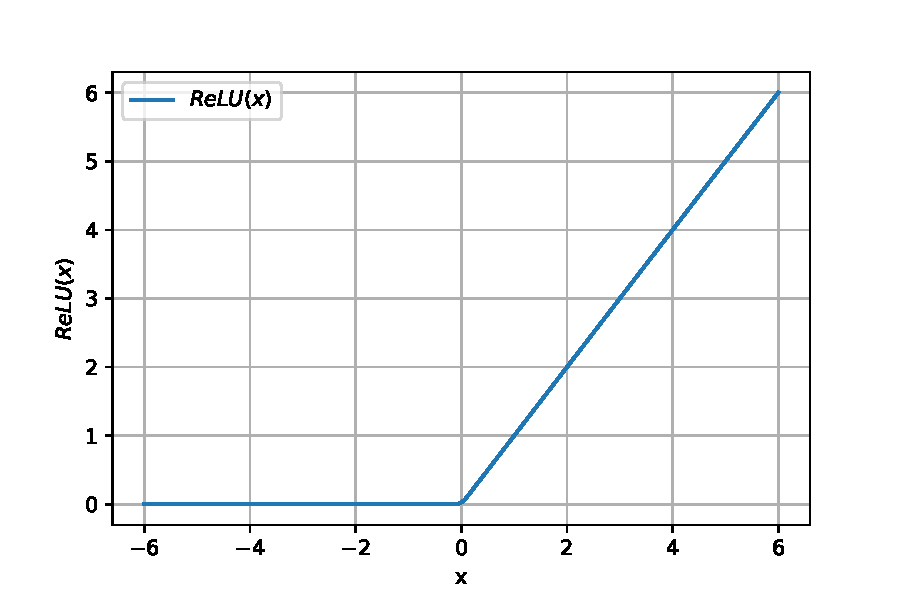
\includegraphics[width=2.7in, fbox]{Chapter2/ReLu.pdf}
        \caption{Rectified Linear Unit (ReLU)}
        \label{fig:relufunc} 
    \end{subfigure}%
    ~
    \begin{subfigure}[b]{0.49\textwidth}
        \centering
        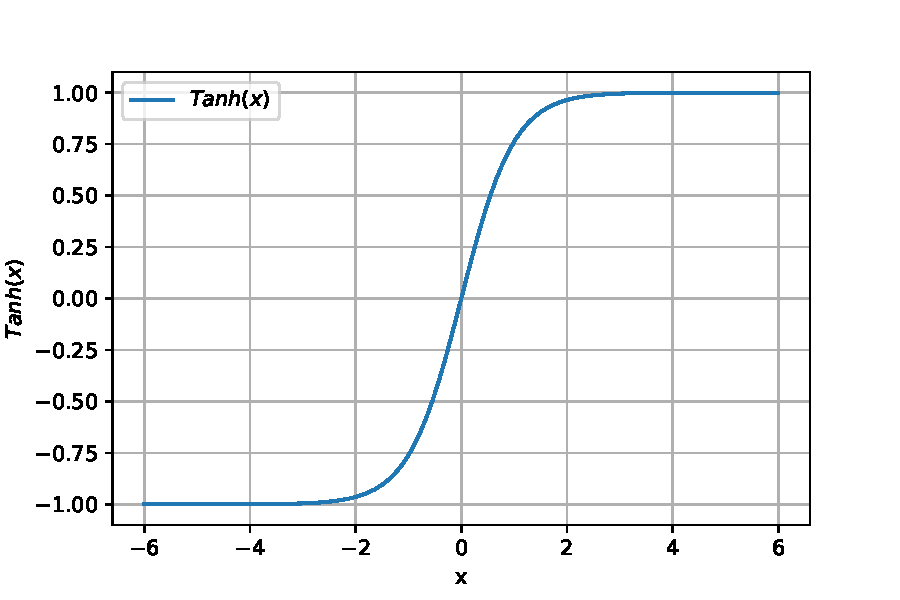
\includegraphics[width=2.7in, fbox]{Chapter2/tanh.pdf}
        \caption{Hyperbolic Tangent (Tanh)}
        \label{fig:tanhfunc} 
    \end{subfigure}
    \caption{Four Common Activation Functions}
    \label{fig:activationfunc} 
\end{figure}

For example, as shown in~\autoref{fig:activationlayer}, the blue line and red line in the input layer represent the input data. The division line is a curve between the two classes. After the activation layer (\textit{Sigmoid} function), the $2-D$ input space is transformed into a $3-D$ shape so that the examples from two classes can be separated linearly (the black line in center image in~\autoref{fig:activationlayer} is the division line)\footnote{This image is edited based on the Christopher Olah's origin version at  \url{http://colah.github.io/posts/2014-03-NN-Manifolds-Topology/}. The author has posted many insightful images, and these images are used by Y.Lecun and Yoshua.B in their publications~\cite{bengio2017deep, lecun2015deep}.}


\begin{figure}[th]
\centering
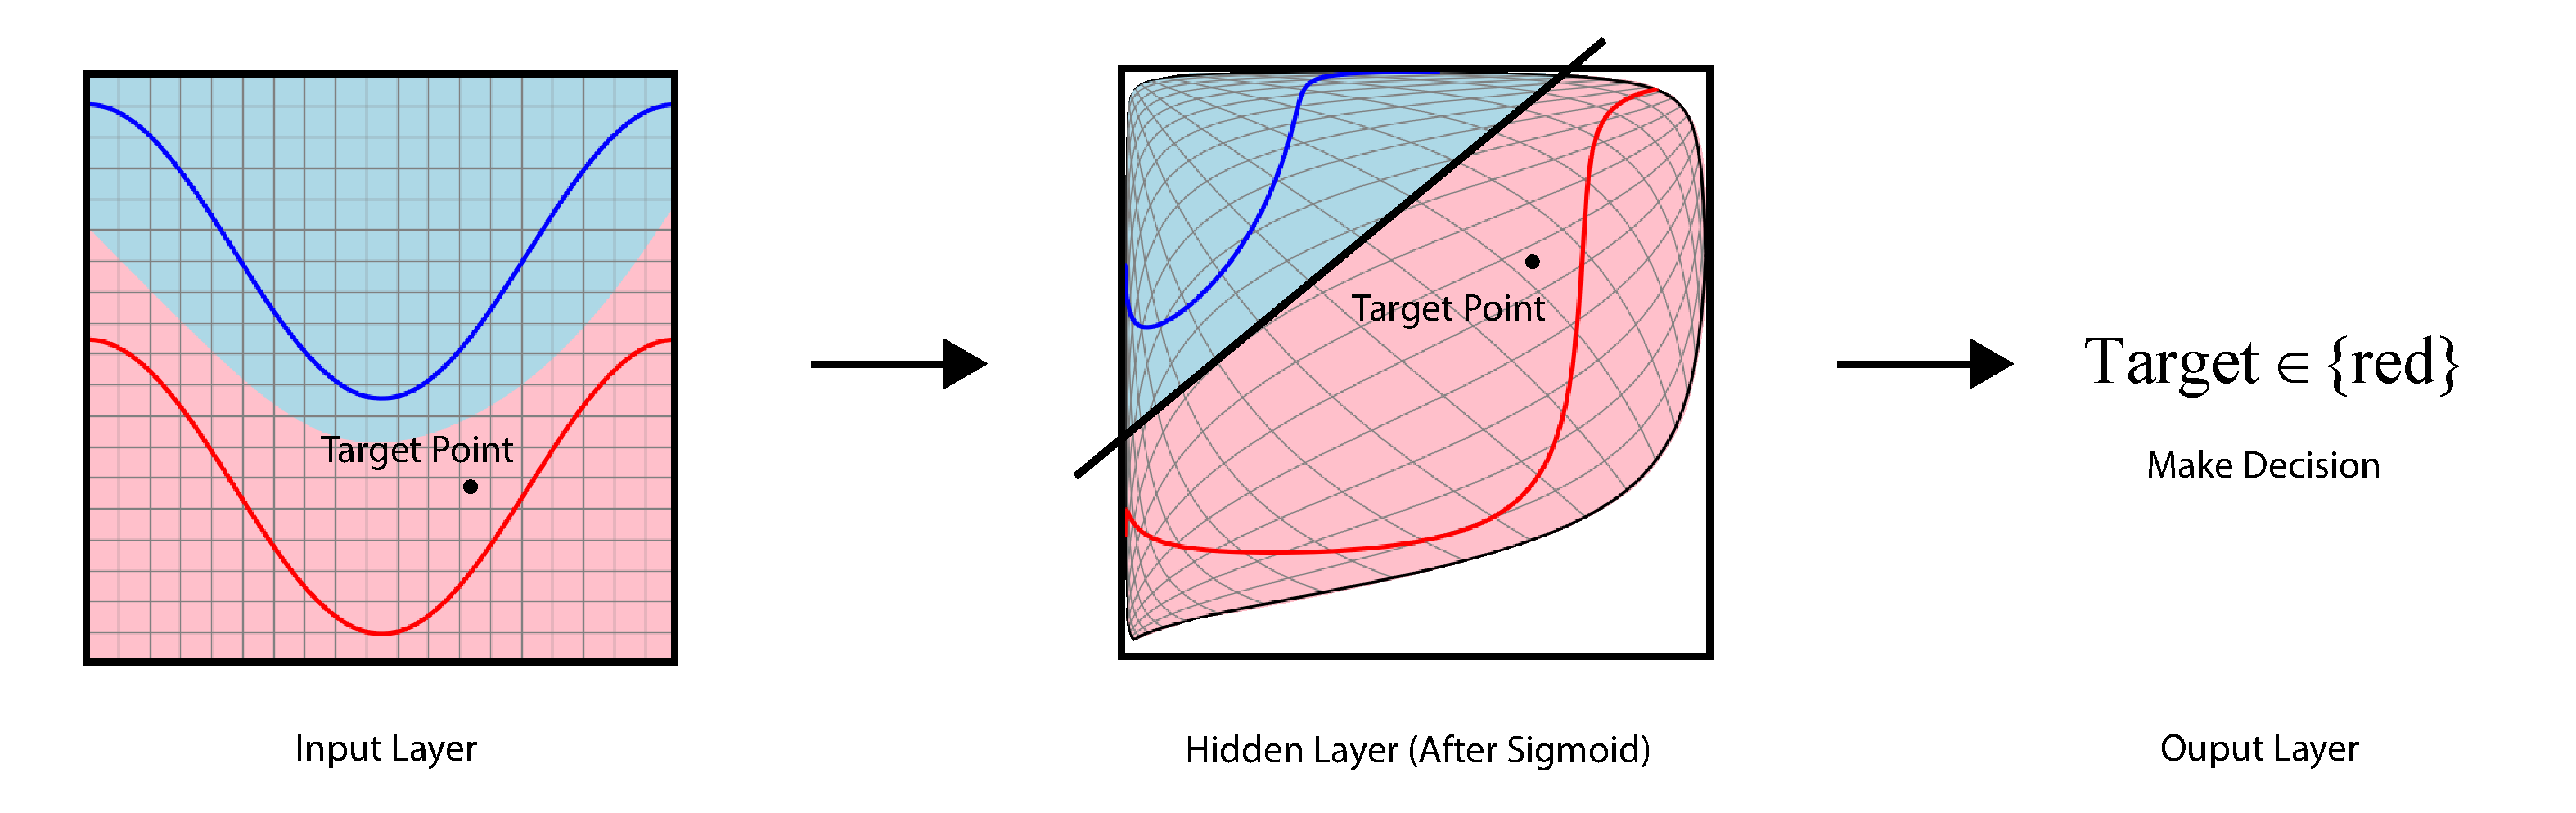
\includegraphics[width=0.99\textwidth, fbox]{Chapter2/activation.pdf}
\caption{Activation Kernal for Linear Decision~\cite{olah2014neural}}
\label{fig:activationlayer} 
\end{figure}

Any single layer in deep learning is made up of non-linear neurons. As shown in~\autoref{fig:simplenn}, the input layer consists of two neurons; the hidden layer (defined as those nodes not input either output) consists of 9 nodes; the output layer consists of only one node. Usually, the output layer may consist of many nodes, in which case the \textit{flatten layer}, \textit{softmax layer} or other logistic regression functions are needed at the end of the neural network to make the output match with the real-world case. Furthermore, the parameter $W_i$, the weight of the $i$-th neuron, is the central part adjusted in the training process. This process is called feed-forward backpropagation, which will be discussed in~\autoref{subsec:back_propagation}.

\begin{figure}[th]
\centering
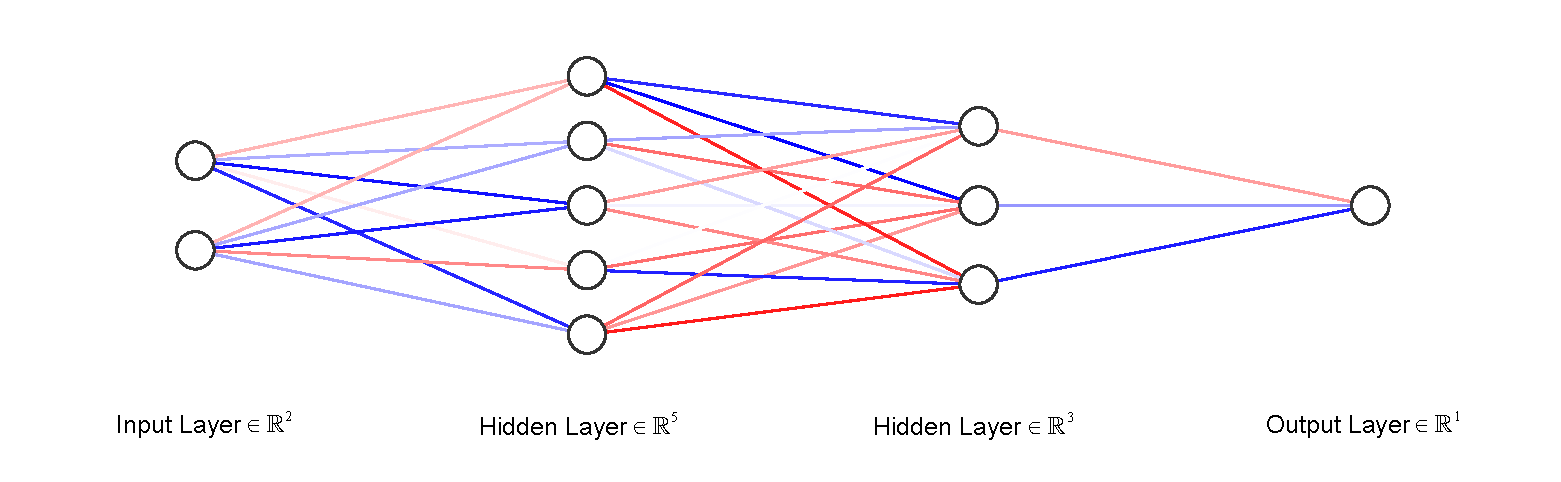
\includegraphics[width=0.99\textwidth, fbox]{Chapter2/simplenn.pdf}
\caption{Simple Neural Network}
\label{fig:simplenn} 
\end{figure}

\subsection{Back Propagation and Feedforward Network}
\label{subsec:back_propagation}

Backpropagation and feedforward are based on the chain rule of derivatives. Below is the basic chain rule. Given \autoref{eq:chainrule1} and \autoref{eq:chainrule2},

\begin{align}
    \Delta z=\frac{\partial z}{\partial y}\Delta y \label{eq:chainrule1}\\
    \Delta y=\frac{\partial y}{\partial x}\Delta x \label{eq:chainrule2}
\end{align}

The \autoref{eq:chainrule3} can be get.

\begin{equation}
\label{eq:chainrule3}
    \frac{\partial z}{\partial x}=\frac{\partial z}{\partial y} \cdot \frac{\partial y}{\partial x}
\end{equation}

One most common and basic feedforward and backpropagation are shown in~\autoref{fig:backpropagation}. It has four layers, the input layer $i$, the hidden layer $j,k$, and the output layer $l$. We use this diagram to explain the feedforward and backpropagation process.

When feeding forward, the input data pass through the activation functions shown in~\autoref{eq:neuralunit} and calculate the output $y_l$. The backpropagation process utilizes the chain rule. The most beginning error gradient is $\frac{\partial E}{\partial y_l}=\Delta y$. With the chain rule, we can see: the error was accumulated along the training path, thus with given activation function, the gradient in each level $G_t,t \in \{i,j,k\}$ can be derived as in~\autoref{eq:backprop} and in~\autoref{fig:backpropagation}.

\begin{equation}
\label{eq:backprop}
    G_t = \frac{\partial E}{\partial z_i},\frac{\partial E}{\partial y_k},\frac{\partial E}{\partial z_k},\frac{\partial E}{\partial y_j},\frac{\partial E}{\partial z_j}
\end{equation}

\begin{figure}[th]
\centering
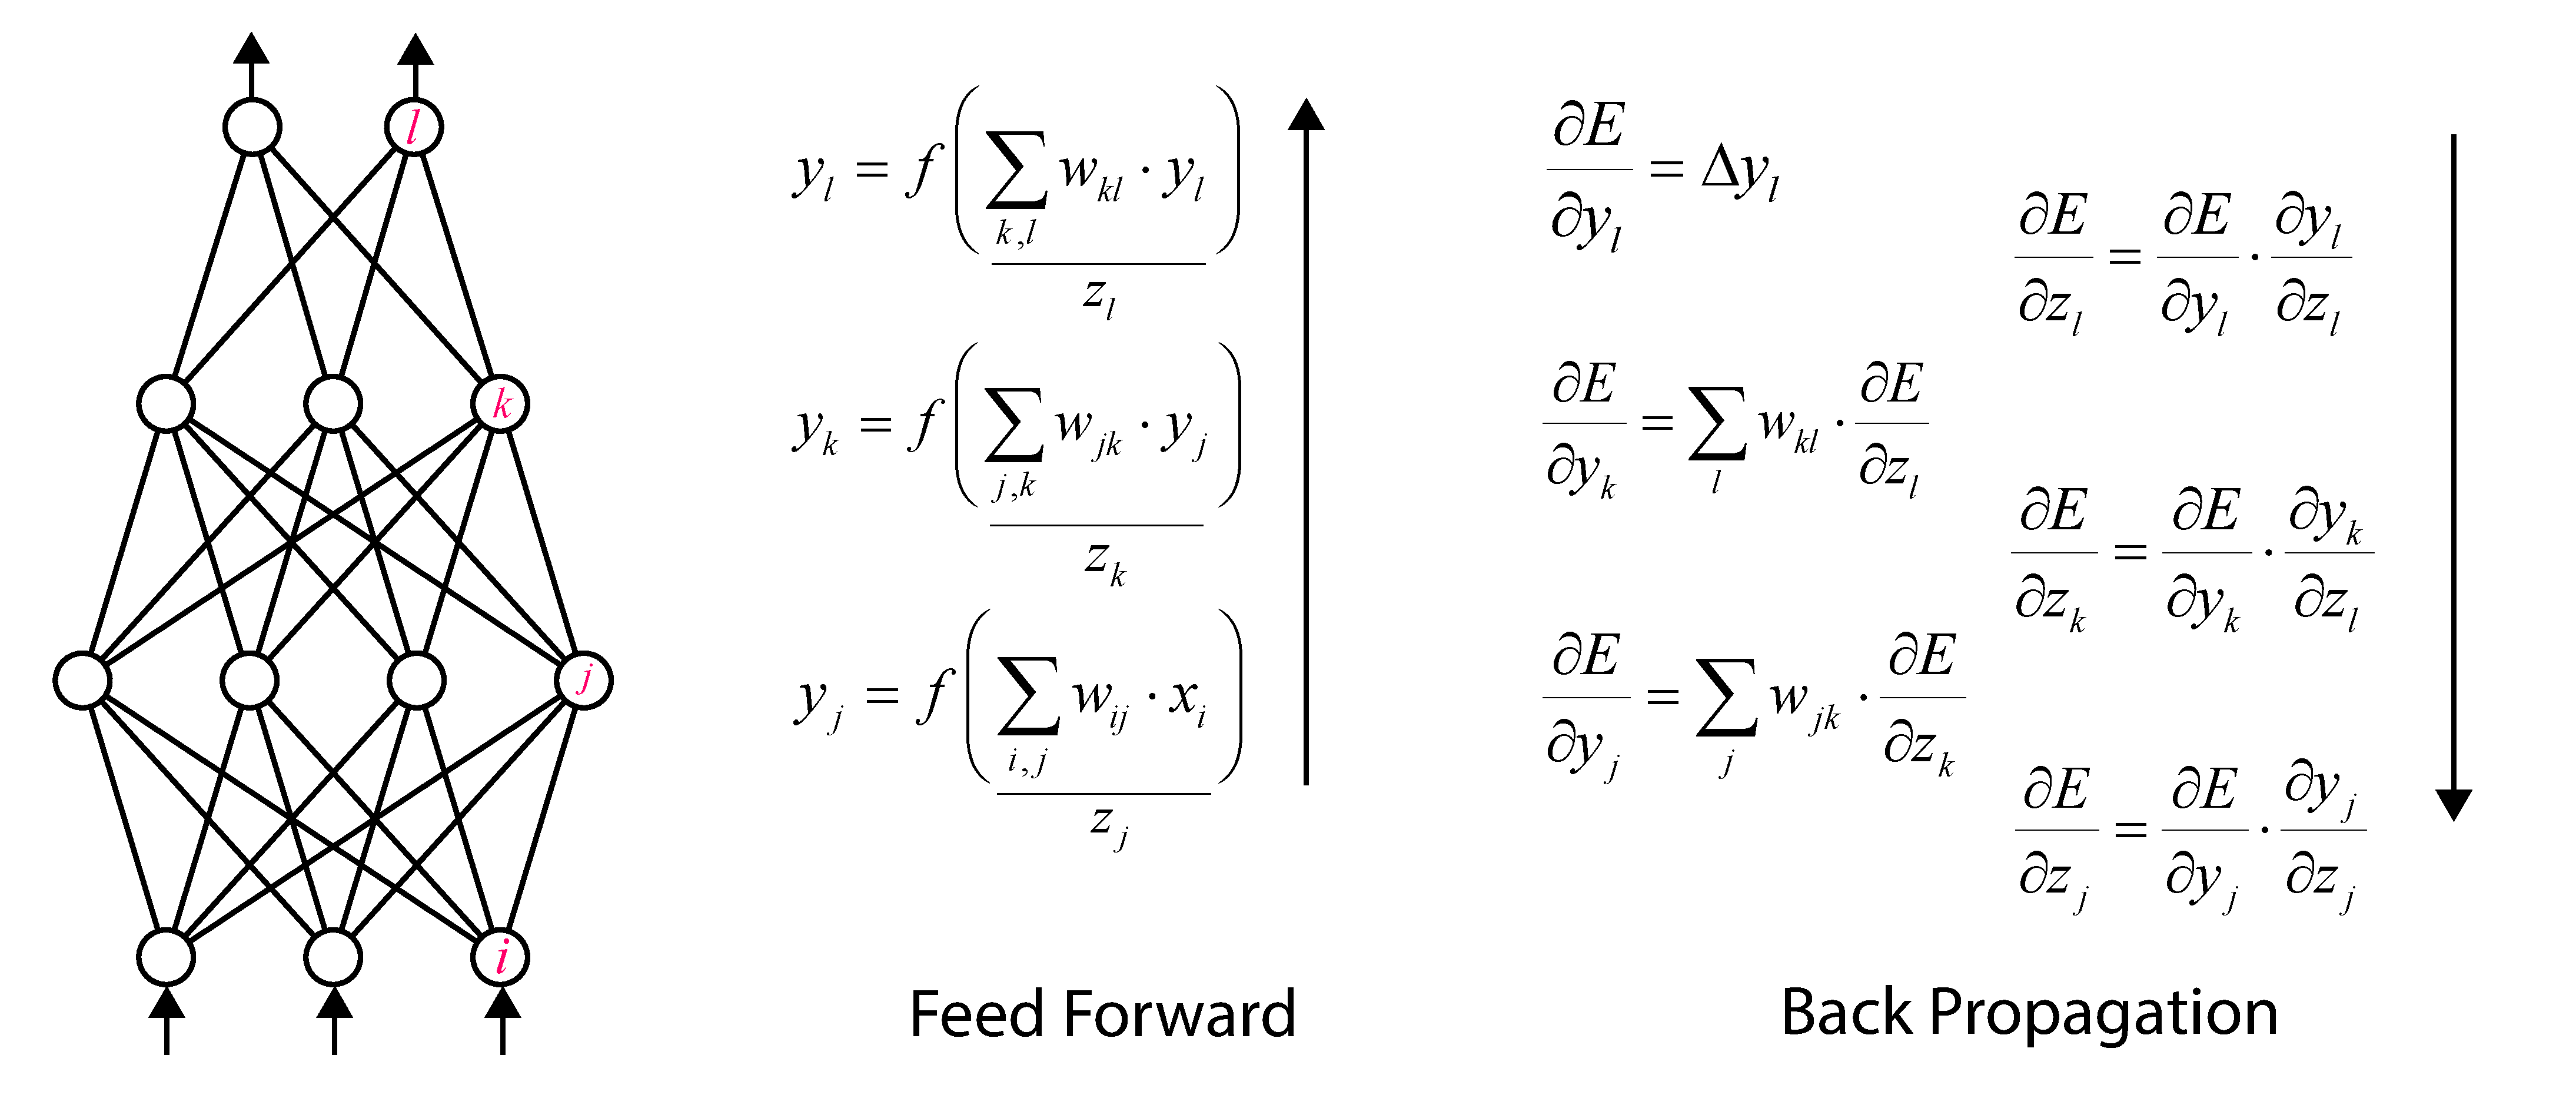
\includegraphics[width=0.99\textwidth, fbox]{Chapter2/backpropagation.pdf}
\caption{Feed Forward and Back Propagation Process}
\label{fig:backpropagation} 
\end{figure}

Notice that the each $G_t(w_{xy})$ is a linear function for weights $w_{xy}$. The aim of model is to minimize the \textit{Error} $E$. To achieve this goal, it is best to go the direction where the gradient $G_t$ decreases fastest, thus the distance $\Delta y=y_t-y_p$ between the ground-truth $y_t$ and the predicted value $y_p$ will shrink in the fastest speed.

In conclusion, the backpropagation can be described as a function $\mathbb{P}$ that

\begin{equation}
    \mathbb{P}=\argmax_{\{w\}}G_t
\end{equation}

\subsection{Application and Growth}

Deep learning is confirmed to be solid in a variety of applications. Due to its good adaption to different source data domains, it can fit any research area rapidly. Some attempts in using deep learning to address the image recognition problem go well above the previous records~\cite{krizhevsky2012imagenet, farabet2012learning, tompson2014joint, szegedy2015going}. Other areas like speech recognition~\cite{mikolov2011strategies, hinton2012deep, sainath2013deep}, natural language understanding (\textit{NLP})~\cite{collobert2011natural}, especially in recognition intelligence, like question responding~\cite{bordes2014question} and translation~\cite{jean2014using, sutskever2014sequence} also have gain surprising results. 

\begin{figure}[ht]
\centering
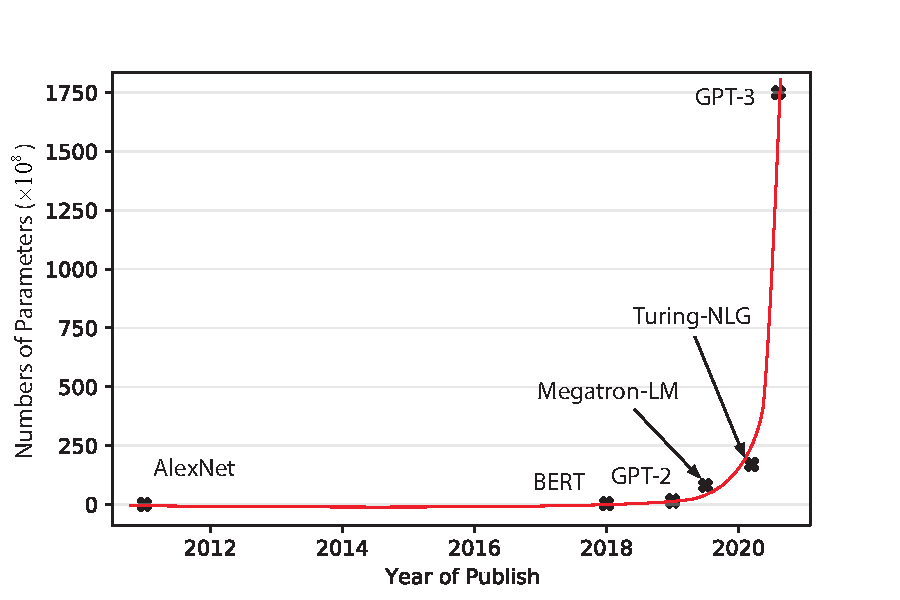
\includegraphics[width=0.99\textwidth, fbox]{Chapter2/paramnum.pdf}
\caption{Parameters of Large Scale Networks}
\label{fig:paramnum} 
\end{figure}

Besides, areas in biomedical, physics, and mathematics are also using deep learning to drive their research. For example, use deep learning to find out the medical-related drug components~\cite{ma2015deep}, to explore the brain circuits~\cite{helmstaedter2013connectomic} and fit the accelerator parameters~\cite{ciodaro2012online}.

The improvements of neural networks are going beyond imagination. Nowadays, researchers are not satisfied with only changing the network structure but are exploring the possibility of extreme-large scale networks. ~\autoref{tab:paramnn} shows recent years' development of frontier models and their neurons used. (More neurons used, more GPU calculation resources needed.) Most recent GPT-3 consists of $1750 \times {10}^8$ parameters, which consumes OpenAI company \textit{12 Million U.S. dollars} for training. It is not realizable for any personal researcher to conduct such a great amount of network. Will the Neural Network's future fall into the control of few big IT companies who can afford such great cost?

\begin{table}[ht]
\caption{Parameter No. of Art-of-state Neural Networks}
\label{tab:paramnn}
\begin{tabular}{cccc}
\toprule
\textbf{Network} & \textbf{Number of Parameters} & \textbf{Area}        & \textbf{Year} \\ \midrule
AlexNet~\cite{krizhevsky2012imagenet}     & $0.6 \times {10}^{8}$ & Image Classification & 2011     \\
BERT~\cite{Jacob2018BERT}        & $3 \times {10}^{8}$   & Language Model       & 2018     \\
GPT-2~\cite{radford2019language}       & $15 \times {10}^{8}$  & Language Model       & 2019     \\
Megatron-LM~\cite{Shoebi2019MegatronLM} & $80 \times {10}^{8}$  & Language Model       & 2019     \\
Turing-NLG~\cite{tnlg}  & $170 \times {10}^{8}$ & Language Model       & 2020.02 \\
GPT-3~\cite{brown2020language}       & $1750 \times {10}^{8}$  & Language Model       & 2020.06 \\ \bottomrule
\end{tabular}
\end{table}

According to DistilBERT~\cite{sanh2019distilbert}, small networks are still more flexible for more application scenarios. \autoref{fig:paramnum} shows the growth of numbers of neural parameters in recent years.

\section{Fully Convolution Networks}
\label{sec:LR_FCN}

A convolutional network is suitable for those deep learning problems related to images.

Traditional Neural Networks perform poorly in image-related areas. In traditional Artificial Neural Networks (ANNs), one neuron in the $n+1$-th layer will be connected to all neurons in the $n$-th layer. When the network scale is small, this can work. However, when the network's input is images, the ANN's full-connection method is inefficient and calculation-consuming. For example, a single RGB image of size $(480 \times 640)$ contains 1,228,800 data units, and each neuron in the hidden layer should have 1,228,800 weights to be calculated.

The convolutional network uses \textit{Convolutional Layer} to avoid the above-mentioned problem. With Convolutional Layer, each neuron only focuses on a limited area on the previous layer, thus reducing the weights in the back-propagation process.

\subsection{Convolutional Layer}

The basic concept of convolutions network was first proposed by Yann Lecun and Yoshua Bengio around 1990s~\cite{bengio1997convolutional, lecun1989backpropagation}. In 2012, the proposal of AlexNet~\cite{krizhevsky2012imagenet} raised the new heat in convolutions networks. Some vital progress is used in AlexNet~\cite{kaiming2014learning}, which makes the convolutional network so effective. That progress includes the proposal of Rectified Linear Unit (ReLU)~\cite{nair2010rectified}, which makes the activation of neurons in the convolutional layer more effective, and the collection of large scale data set~\cite{deng2009imagenet}, which make the networks being fully trained.


\begin{figure}[ht]
\centering
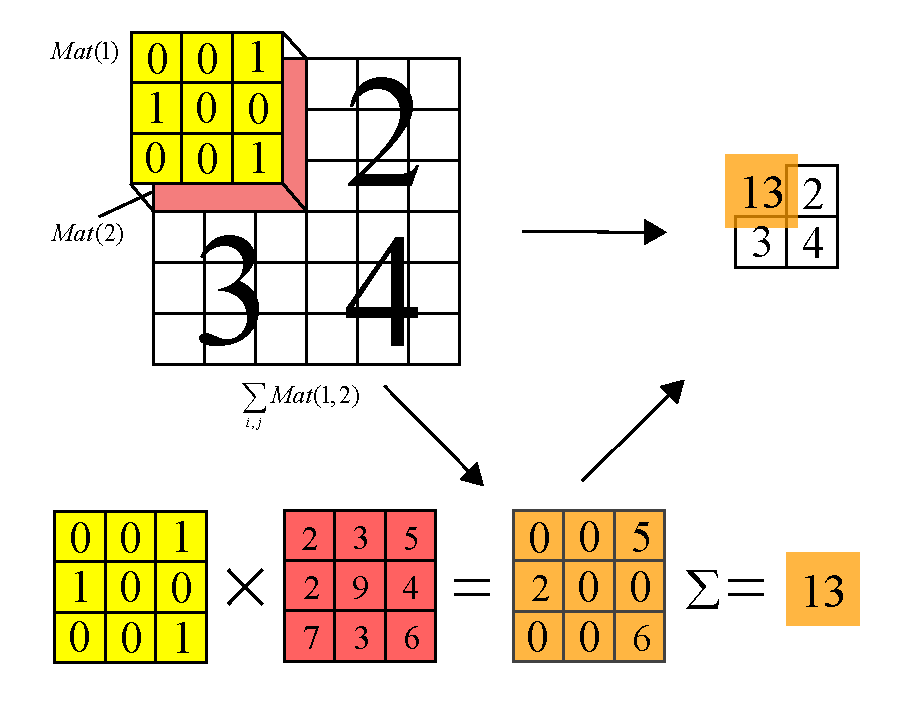
\includegraphics[width=0.99\textwidth, fbox]{Chapter2/2dconv.pdf}
\caption{$2-D$ Convolution in 1 Channel}
\label{fig:2dconv} 
\end{figure}

Convolutional layers are mainly used to address the pattern recognition and classification problems related to images~\cite{o2015introduction}. The convolutional layer does $2-D$ convolution to the given input image, and the convolutional kernel will become the weights of the neurons. When training the convolutional network with backpropagation, the weights (parameters in the convolutional kernel) are optimized from time to time.

Begin with a 1-channel $2-D$ convolution. $2-D$ convolution is given in~\autoref{eq:2dconv}.

\begin{equation}
\label{eq:2dconv}
    y[i,j]= \sum_m \sum_n h[m,n] \cdot x[i-m,j-n]
\end{equation}

For clearer explanation, the process is shown in \autoref{fig:2dconv}, the $2-D$ convolutional kernel is the $Mat(1)$. Put the $Mat(1)$ at the upper-left corner and do pixel-wise adding. The sum of the result would become the upper-left element in the output matrix (The orange element in \autoref{fig:2dconv}). In a nutshell, $2-D$ convolution is to identify intensity changes within a local neighbourhood of pixels. Then, a single pixel value encodes this information, thereby describing the local neighbourhood.

The convolution layer is constructed by the neurons described in~\autoref{subsec:neural_unit}. Each convolutional kernel are $(n \times n \times depth)$ matrix, in which $depth$ is the number of channels of the input image. For RGB image, $depth = 3$. \autoref{fig:convtoneuron} shows how the two things are related together. The kernel size in the diagram is $(n \times n \times 3)$. After flatten, the neuron function $\Phi(x)$ will get $(n \times n \times 3)$ weights, and produce $1$ output $\beta_1$. Usually, in one convolutional layer, there are more then one neurons, thus the figure also contains $\beta_2, \beta_3, ..., \beta_k$. They are generated by other neurons $\Phi_2(x), \Phi_3(x), ..., \Phi_k(x)$.

\begin{figure}[ht]
\centering
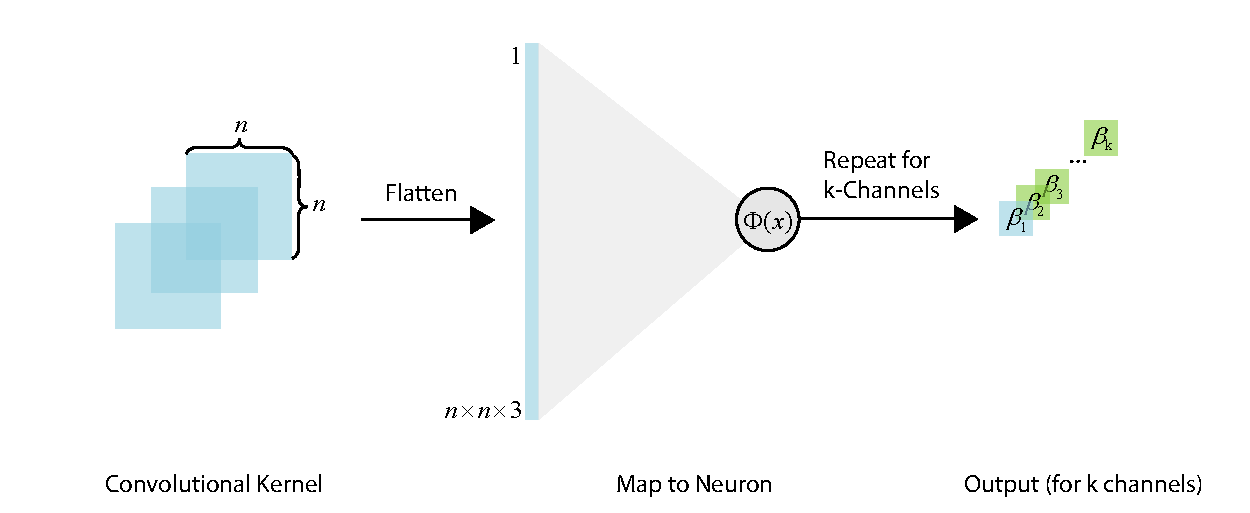
\includegraphics[width=0.99\textwidth, fbox]{Chapter2/convtoneuron.pdf}
\caption{How $2-D$ Convolutional Layer Related with Neuron}
\label{fig:convtoneuron} 
\end{figure}

\autoref{fig:multineuron} gives more clearer explanation of the situation that multi kernels are used.

\begin{figure}[ht]
\centering
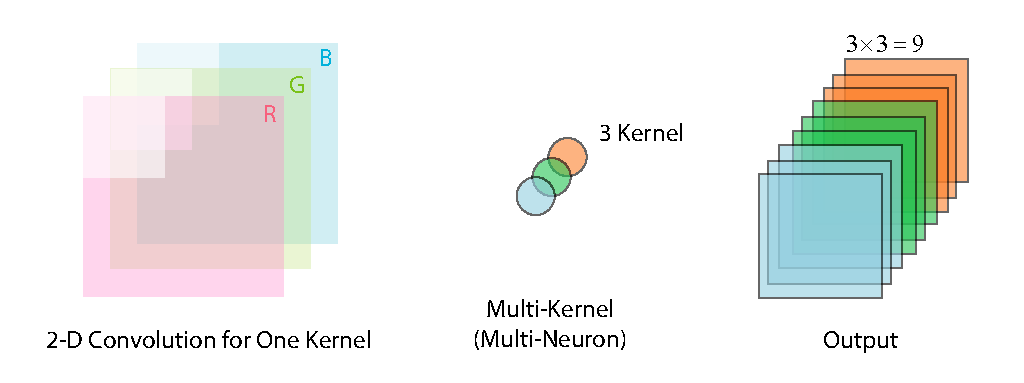
\includegraphics[width=0.99\textwidth, fbox]{Chapter2/multineuron.pdf}
\caption{Multi-neuron Output}
\label{fig:multineuron} 
\end{figure}

\subsection{Some Common Conception}

\textbf{Image} refer to $2-D$ or $n-D$ matrix containing pixels, depends on the image presenting method (RGB, CMYK, HSB, and HSL etc.) In the following description, it is assumed that a RGB image is used. Each RGB image contains $(n \times m)$ pixels, and each pixel are represented by $(R,G,B)$ three channels (stands for (Red, Green, Blue)). Usually, in the digital image saving, each channel for each pixel saves an \textit{int}\footnote{For different standards, the saved data type is different, \texttt{uint8}, \texttt{uint32} and \texttt{float} are most common ones.} type value. For example, given a $(480 \times 640)$ RGB image, it contains $(480 * 640 * 3)=1,228,800$ \textit{int} values.

\textbf{Receptive field size} is the area that a single pixel in output reflects in the input. The size of receptive field is determined by the convolutional kernel size, the stride and the padding of kernel. A very simple example is shown in \autoref{fig:convtoneuron}: after the convolutional layer, a $(n \times n)$ area will be mapped into only $1$ pixel. For pixel $\beta_1$, the receptive field size is $(n \times n)$. If this process goes twice (the input image goes through two convolutional layers shown in \autoref{fig:convtoneuron}), single pixel in thee output will have receptive field of $(n \times n)^2=n^4$ pixels size.

\section{Concluding Remarks}

This chapter first reviewed the history and recent progress in lane detection algorithms. Second, it introduced several machine learning types and their differences. Third, it introduced the main kinds of deep learnings and their differences. 

After the introduction, neural networks' theoretical basis is described, from the most basic structure: neurons, to high-level structure: convolutional layers.

The following section will focus on the RVPGNet lane detection algorithm based on the FCN network.

%=== END OF CHAPTER TWO ===
\end{spacing}
\newpage
